\chapter{Derivation of Ramsey's Method}
\textbf{MUST BE EDITED} In this section, we'll review the Ramsey
technique for molecular beam resonance experiments. In all previous
studies the oscillating fields were extended approximately uniformly
throughout the regions in which the energy levels of the system were
investigated. This was not efficient since the amplitude and phase of
the oscillating field might change along the path of the beam. As a
different approach, Ramsey suggested to confine the oscillating fields
to small regions; one at the beginning of the space which the energy
levels are being studied and the other one at the end. In this case,
there is no oscillating field in between.

Consider a system which at time $t_1$ is subjected to an oscillatory
perturbation which induces transition between eigenstates p and q:
\begin{equation}
V=
\left(
\begin{array}{cc}
0 & \hbar b e^{i\omega t} \\ 
\hbar b e^{-i \omega t} & 0
\end{array} 
\right)
\end{equation}
An example of such perturbation is a system with a magnetic moment
entering a region with rotating magnetic field with angular velocity
$\omega$. The general wave function for this system is :
\begin{equation}
\psi(t)= C_p (t) \psi_p + C_q(t) \psi_q
\end{equation}
Therefore, the time dependent Schr\"{o}dinger equations will have the
form :

\begin{align}
\left\lbrace
\begin{array}{cc}
i \hbar \dot{C}_p(t)&= W_p C_p(t)+\hbar b e^{i \omega t} C_q(t) \\
i \hbar \dot{C}_q(t)&=\hbar b e^{-i \omega t} C_p(t) +W_q C_q(t)
\end{array}
\right.
\end{align}
Let's write the above equation in matrix notation and solve for
$C_p(t)$ and $C_q(t)$. Let's define

\begin{equation}
C= \left(
\begin{array}{cc}
C_p \\
C_q
\end{array} \right)
\end{equation}
Hence, we would get,
\begin{equation}
i \hbar \frac{d}{dt}\left(
\begin{array}{cc}
C_p \\
C_q
\end{array} \right) =
\left(
\begin{array}{cc}
W_p & \hbar b e^{i \omega t} \\
\hbar b e^{-i \omega t} & W_q 
\end{array} \right)
\left(
\begin{array}{c}
C_p \\
C_q
\end{array}\right)
\end{equation}
We assume that, at $t=t_1$, $C_p$ and $C_q$ have the values $C_p(t_1)$
and $C_q(t_1)$ respectively. We are interested in the solution of the
above equation at $t=t_1+T$. The matrix on the right side can be
written as
\begin{align}
\left(
\begin{array}{cc}
W_p & \hbar b e^{i\omega t} \\
\hbar b e^{-i\omega t} & W_q 
\end{array}
\right) &=
\left(
\begin{array}{cc}
W_p & \hbar b \cos{\omega t}+i \hbar b \sin{\omega t} \\
\hbar b \cos{\omega t}-i \hbar b \sin{\omega t} & W_q
\end{array}
\right) \\
&= \left(
\begin{array}{cc}
W_p & 0 \\
0 & W_q
\end{array} \right) -\hbar b \sin{\omega t} \sigma_2 +\hbar b \cos{\omega t} \sigma_1
\end{align}
Where $\sigma_1$ and $\sigma_2$ are Pauli matrices. Hence, The time
dependent Schr\"{o}dinger equation will take the form
\begin{equation}
\frac{d}{dt} \left( \begin{array}{c}
C_p \\
C_q
\end{array}\right) =
-i \left[
\left(
\begin{array}{cc}
\frac{W_p}{\hbar} & 0 \\
0 & \frac{W_q}{\hbar}
\end{array}\right)
+ b \sigma_1\cos{\omega t}  -b \sigma_2 \sin{\omega t} 
\right]\left( \begin{array}{c}
C_p \\
C_q
\end{array}\right)
\end{equation}
But, we can rewrite the first matrix on the right side as
\begin{equation}
\left( \begin{array}{cc}
\frac{W_p}{\hbar} & 0 \\
0 & \frac{W_q}{\hbar}
\end{array} \right) = \left(
\begin{array}{cc}
\frac{W_p+W_q}{2\hbar} + \frac{W_p-W_q}{2\hbar} & 0 \\
0 & \frac{W_p+W_q}{2\hbar}-\frac{W_p-W_q}{2\hbar}
\end{array} \right)
\end{equation}
Let's define
\begin{equation}
C=\left( \begin{array}{c}
C_p \\
C_q
\end{array}\right) , 
\Omega=\frac{W_p+W_q}{2\hbar} ,
\omega_0=\frac{W_q-W_p}{\hbar}
\end{equation}
Therefore the Schr\"{o}dinger equation takes the form
\begin{equation}
\frac{d}{dt}C= -i \left[
\Omega -\frac{\omega_0}{2}\sigma_3 + b \left(\sigma_1 \cos{\omega t}  - \sigma_2\sin{\omega t}  \right) \right]\left( \begin{array}{c}
C_p \\
C_q
\end{array} \right)
\end{equation}
The term $\left( \sigma_1\cos{\omega t}  - \sigma_2 \sin{\omega t}  \right)$ is like a rotation. In general, we have
\begin{equation}
e^{-i \vec{\sigma}\cdot\hat{n} \frac{\theta}{2}} \vec{a}. \vec{\sigma} e^{i \vec{\sigma}.\hat{n} \frac{\theta}{2}}=\left[ \hat{n}(\hat{n}.\vec{a})+\cos\theta (\vec{a} - \hat{n} (\hat{n}.\vec{a}))+\sin \theta (\hat{n} \times \vec{a} )\right] \vec{\sigma} .
\end{equation}
If we consider $\hat{n}=-\hat{k}$ and $\vec{a}=\hat{x}$, then we would
get
\begin{equation}
\sigma_1 \cos{\omega t} - \sigma_2 \sin{\omega t} = e^{i \frac{\omega t}{2} \sigma_3} \sigma_1 e^{-i \frac{\omega t}{2}\sigma_3} .
\end{equation}
Hence, the Schr\"{o}dinger equation will take the form 
\begin{equation}
\dot{C}= -i e^{ i \frac{\omega t}{2}\sigma_3} \left[\Omega - \frac{\omega_0}{2} \sigma_3+b \sigma_1\right] e^{-i\frac{\omega t}{2}\sigma_3} C .
\end{equation}
Let's define D as
\begin{equation}
C= e^{i \frac{\omega t}{2}\sigma_3} e^{-i \Omega t} D
\end{equation}
Now, we rewrite the Schr\"{o}dinger equation in terms of variable D
\begin{equation}
\dot{D}=-i \left[ \left( \frac{\omega - \omega_0}{2}\right) \sigma_3 +b \sigma_1 \right]D ,
\end{equation}
and by defining
$ a:= {\left[{(\omega_0 - \omega)}^2+ {(2b)}^2\right]}^\frac{1}{2}$ ,
$\cos \theta = \frac{\omega_0 - \omega}{a}$ and
$\sin \theta=\frac{2b}{a}$, we get
\begin{equation}
\dot{D}=\frac{i a}{2}\left[ \sigma_3 \cos \theta - \sigma_1 \sin \theta \right] D .
\end{equation}
Hence, the solution of the above equation has the form
\begin{equation}
D(t_1+T)= e^{\left[\frac{i a}{2}
\left( \sigma_3 \cos \theta
-\sigma_1\sin \theta 
\right) T 
\right]
}D(t_1) .
\end{equation}
If we use \,
$ e^{i \vec{\sigma}\cdot\hat{n}\frac{\phi}{2}}= I \cos \frac{\phi}{2}+
i (\vec{\sigma}\cdot\hat{n})\sin \frac{\phi}{2}$ \, with \, $ \phi=aT$
\, and \,
$\vec{\sigma}\cdot\hat{n}=\sigma_3 \cos \theta -\sigma_1 \sin \theta$,
then
\begin{equation}
D(t_1+T)= \left[\cos \frac{aT}{2}+i(\sigma_3 \cos \theta - \sigma_1 \sin \theta ) \sin \frac{aT}{2}\right] D(t_1)
\end{equation}
and therefore $C(t_1+T)$ would be
\begin{equation}
C(t_1+T)= e^{i\frac{\omega}{2}(t_1+T)\sigma_3} e^{-i \Omega T} \left[\cos \frac{aT}{2}+i(\sigma_3 \cos \theta - \sigma_1 \sin \theta ) \sin \frac{aT}{2}\right] e^{-i \frac{\omega t_1}{2}\sigma_3} C(t_1),
\end{equation}
or equivalently
\begin{equation}
\left\lbrace
\begin{array}{c}
  C_p(t_1+T)= \left\lbrace \left[
  i \cos \theta \sin \frac{aT}{2}+\cos \frac{aT}{2} \right] C_p(t_1)-
  \left[i \sin \theta \sin \frac{aT}{2} e^{i \omega t_1} \right]C_q(t_1)\right\rbrace \times \\
  e^{\left\lbrace i\left[\frac{1}{2}\omega - \frac{(W_p + W_q)}{2\hbar}\right] T\right\rbrace}
  \\
  \, \,
  \\
  C_q(t_1+T)=\left\lbrace - \left[ i \sin \theta \sin \frac{aT}{2} e^{-i \omega t_1}\right]C_p(t_1) +
  \left[-i \cos \theta \sin \frac{aT}{2}+ \cos \frac{aT}{2}\right] C_q(t_1)\right\rbrace \times
  \\
  e^{\left\lbrace i \left[ -\frac{\omega}{2}- \frac{W_p+W_q}{2\hbar} \right] T \right\rbrace}
\end{array}
\right. .
\end{equation} 
These are the general solutions for a system with energy eigenstates
$p$ and $q$. As a comparison, if we put $C_p(t_1+T)=a(t)$ ,
$C_q(t_1+T)=b(t)$, $a= \omega'$ , $2b=\omega_1$ then we would get
equation (1.31). In this case, $W_p$ and $W_q$ are energies of the
spin up and spin down configurations.
\\
As a special case, if b=0 (no perturbation), then $\cos \theta=1$ and
$\sin \theta=0$. Hence, the solutions would be
\begin{equation}
\left\lbrace
\begin{array}{c}
C_p(t_1+T)= e^{-i \frac{W_p}{\hbar} T} C_p(t_1) \\
C_q(t_1+T)=e^{-i \frac{W_q}{\hbar}T} C_q(t_1)
\end{array}
\right. .
\end{equation}
%
Now, consider a system which is subjected to perturbation for time
$\tau$ and length $l$, then the perturbation goes off for time $T$ and
length $L$ and again the perturbation goes on for another time
$\tau$. To achieve greater generality, corresponding to the
experimental impossibility of attaining completely uniform magnetic
fields, we assume that energy levels $p$ and $q$ are not constant in
the intermediate state when b=0, which means it is divided to
sub-regions with duration $\Delta t_k$ and energies are $W_{p,k}$ and
$W_{q,k}$ respectively. We assume
\begin{equation}
C_p(0)=1 , \, \, C_q(0)=0 ,
\end{equation}
which means the system is at state $p$ before it enters the first
perturbation region. Hence, the amplitudes would be
\begin{equation}
\left\lbrace
\begin{array}{c}
C_p(\tau)=\left[i \cos \theta \sin \frac{a\tau}{2}+ \cos \frac{a\tau}{2}\right]
e^{i\left[\frac{\omega}{2}-\left(\frac{W_p+W_q}{2\hbar}\right)\right]\tau}\\
C_q(\tau)=\left[ -i \sin \theta \sin \frac{a\tau}{2} \right] 
e^{i \left[ -\frac{\omega}{2} - \left( \frac{W_p+W_q}{2\hbar}\right)\right]\tau}
\end{array}\right. .
\end{equation}
After entering the intermediate region we would get
\begin{align}
C_p(\tau+T)&=\Pi_k e^{-i W_{p,k} \Delta \frac{t_k}{\hbar}}  C_p(\tau)\nonumber \\
&=e^{-\frac{i}{\hbar} \Sigma_k W_{p,k} \Delta t_k}  C_p(\tau) \nonumber\\
C_p(\tau+T)&=e^{-i \frac{\bar{W_p}T}{\hbar}} C_p(\tau) \\
\nonumber\\
C_q(\tau+T)&=e^{-i \frac{\bar{W_q}T}{\hbar}} C_q(\tau) .
\end{align}
%
It is impossible to have completely uniform magnetic fields in the
experiment. Hence, we assume that the energies of the $p$ and $q$
states are not constant in this region, and the region is divided into
a number of sub-regions such that in the $k^{th}$ sub-region of
duration $\Delta t_k$ the energies are $W_{p,k}$ and $W_{q,k}$.

Here we have,
$\bar{W_p}=\frac{1}{T}\Sigma_k W_{p,k}\Delta t_k=\frac{1}{L}\Sigma_k
W_{p,k} \Delta L_k$, which is the space mean value of $W_p$. There is
a similar interpretation for $W_q$ as well. After entering the final
perturbation region,
\begin{equation}
\left\lbrace
\begin{array}{c}
  C_p(2\tau+T)=\left\lbrace \left[i \cos \theta \sin \frac{a\tau}{2}+\cos \frac{a\tau}{2}\right]C_p(\tau+T) -
  \left[i \sin \theta \sin \frac{a\tau}{2} e^{i \omega (\tau+T)}\right]C_q(\tau+T)\right\rbrace \times
  \\
  e^{i\left[\frac{\omega}{2}-\frac{(W_p+W_q)}{2\hbar}\right]\tau}\\
  \,
  \\
  C_q(2\tau+T)=\left\lbrace -\left[i \sin \theta \sin \frac{a\tau}{2} e^{-i \omega (\tau+T)}\right]C_p(\tau+T)+\left[ -i \cos \theta \sin \frac{a\tau}{2}+ \cos \frac{a\tau}{2}\right] C_q(\tau+T)\right\rbrace \times \\
  e^{i \left[\frac{-\omega}{2}-\frac{(W_p+W_q)}{2\hbar}\right]\tau}
\end{array}
\right.
\end{equation}
We can rewrite the above equation as
\begin{align}
  C_q(2\tau+T)&= 2i\sin \theta \left[ \cos \theta \sin^2 \frac{a\tau}{2}\sin \frac{\lambda T}{2} -\frac{1}{2}\sin a\tau \cos \frac{\lambda T}{2} \right] \nonumber \\ &\times e^{-i \left[\frac{\omega}{2} + \frac{(W_p+W_q)}{2\hbar}\right]}(2\tau+T) +
                                                                                                                                                                        \left[ \frac{\bar{W_p}-W_p+\bar{W_q}-W_q}{2\hbar} 
                                                                                                                                                                        T\right] ,
\end{align} 
where
\begin{equation}
\lambda= \left( \frac{\bar{W_q}-\bar{W_p}}{\hbar} \right)- \omega .
\end{equation}
Therefore, the probability that the system changes from state p to
state q is
%
\begin{equation}
P_{p,q}=|C_q|^2 =4 \sin ^2 \theta \sin ^2 \frac{a\tau}{2} \left[
\cos \frac{\lambda T}{2} \cos \frac{a\tau}{2} -
\cos \theta \sin \frac{\lambda T}{2} \sin \frac{a\tau}{2} \right] ^2 .
\end{equation}
%
We can define a dimensionless parameter
%
\begin{equation}
x:= \frac{\omega_0 - \omega}{2b} , 
\end{equation}
and therefore, $a$ would take the form 
\begin{equation}
a= 2b \sqrt{1+x^2} .
\end{equation}
If we set $b\tau = \frac{\pi}{4}$ (which is similar to the previous
section which $\omega_1 t= \pi$) and $T=8\tau$, then
%
\begin{equation}
P(x)= \frac{4}{1+x^2} \left[ \sin ( \sqrt{1+x^2 \frac{\pi}{4}}) \right]^2
\left[
\cos (2 \pi x) \cos (\sqrt{1+x^2 \frac{\pi}{4}}) - \frac{x}{1+x^2} \sin ( \sqrt{1+x^2 \frac{\pi}{4}}) \right] ^2 ,
\end{equation}
%
and is plotted in Fig. \ref{fig:transprob}.
% 
\begin{figure}[h]
  \centering
    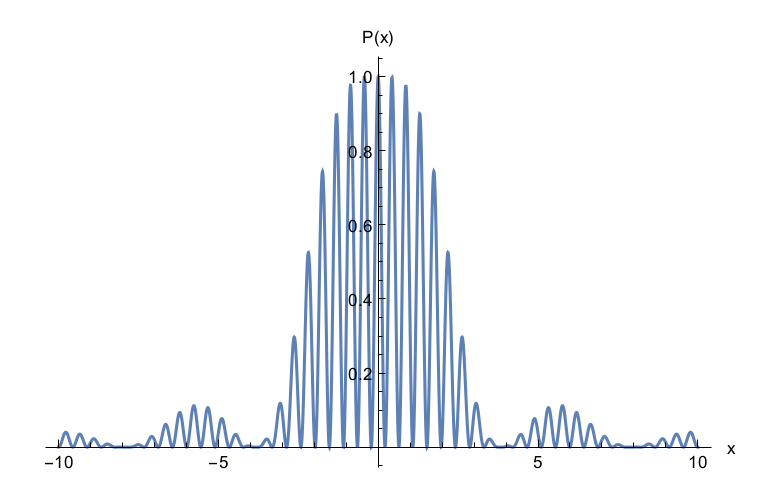
\includegraphics[width=.6\textwidth]{p.pdf}
    \caption{ The graph above shows the transition probability of spin
      down using Ramsey technique of separated oscillating fields. In
      this graph $T=8\tau$ and $ b \tau = \frac{\pi}{4}$. }
    \label{fig:transprob}
\end{figure}
%
An important special case of this relation is that corresponding to a
nuclear magnetic moment of spin-$\frac{1}{2}$ with gyromagnetic ratio
$\gamma$, in a fixed field of strength $B_0$, with a weak field of
strength $B_1$ perpendicular to $B_0$ and rotating about $B_0$. In
this case, the above equation applies with
\begin{align}
\omega_0 &= \gamma B_0 \, , \lambda=\omega_0 - \omega \\
2b &= \gamma B_1 =\frac{\omega_0 B_1}{B_0}
\end{align}
